\mychapter{3}{Applications}

\section{Homology modelling of domains and domain interactions of the human proteome}

\begin{figure}[H]
	\centering
	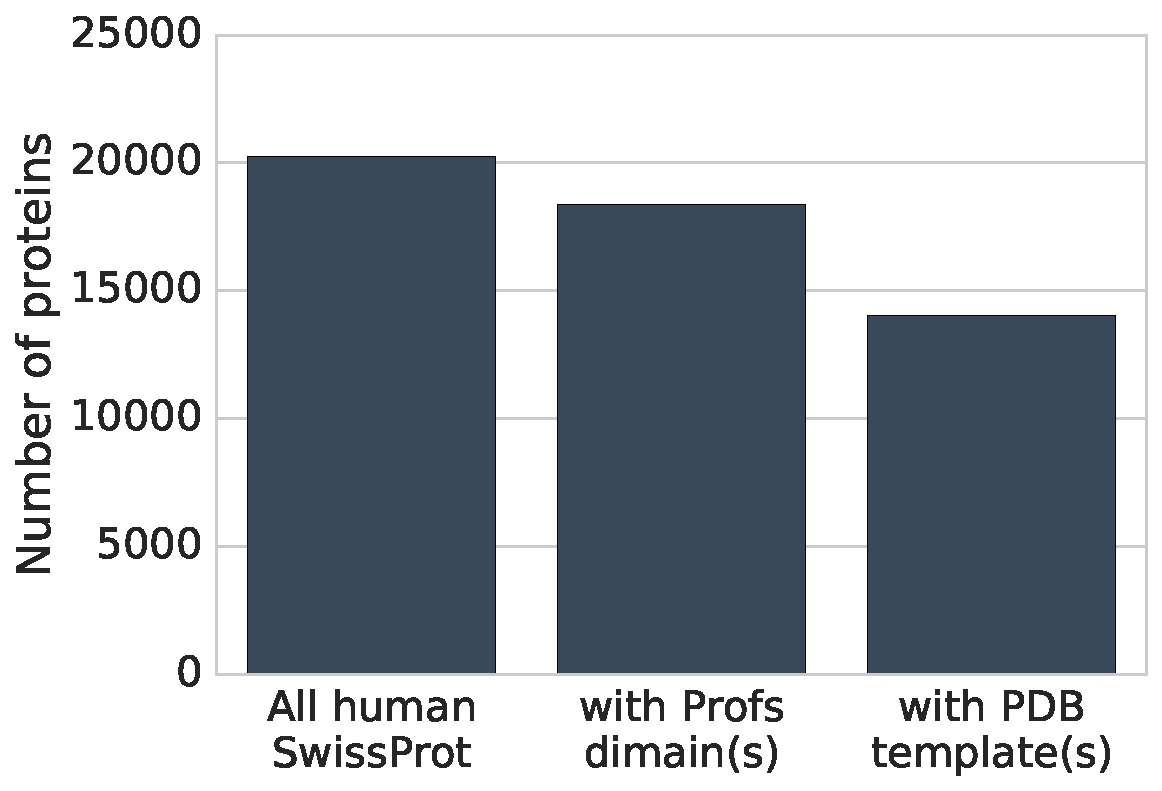
\includegraphics[scale=0.3]{elaspic_statistics/missing_template}
	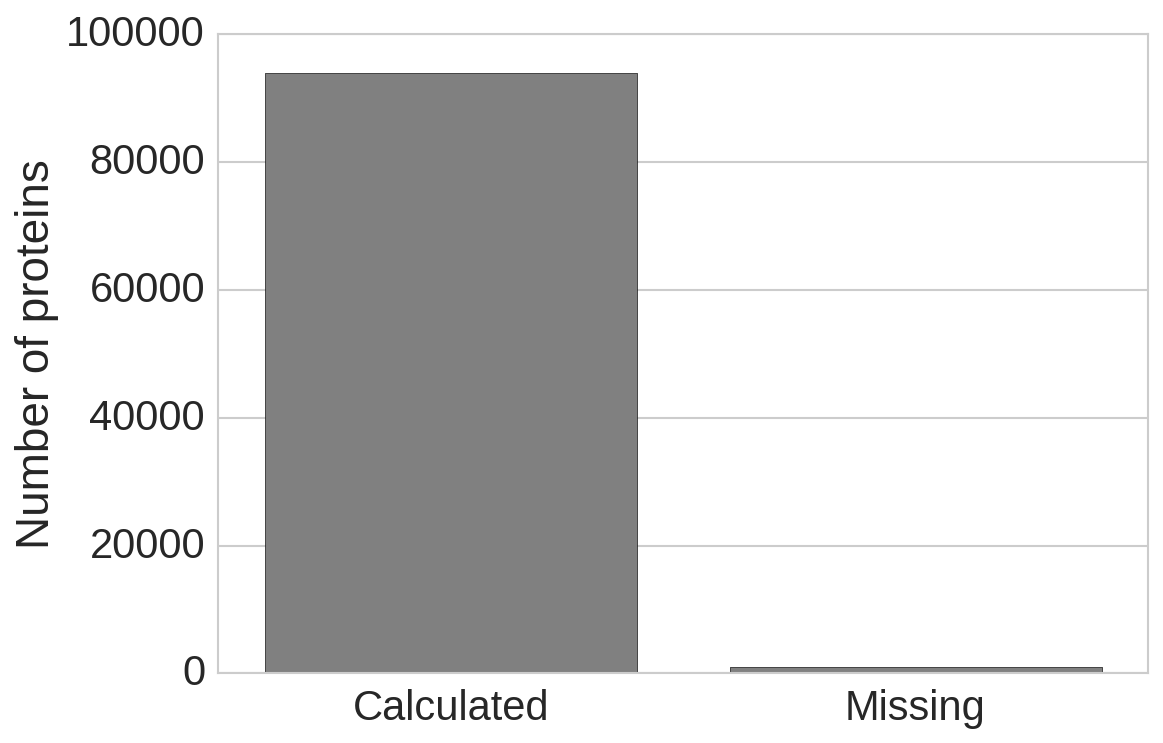
\includegraphics[scale=0.3]{elaspic_statistics/missing_model_protein}
	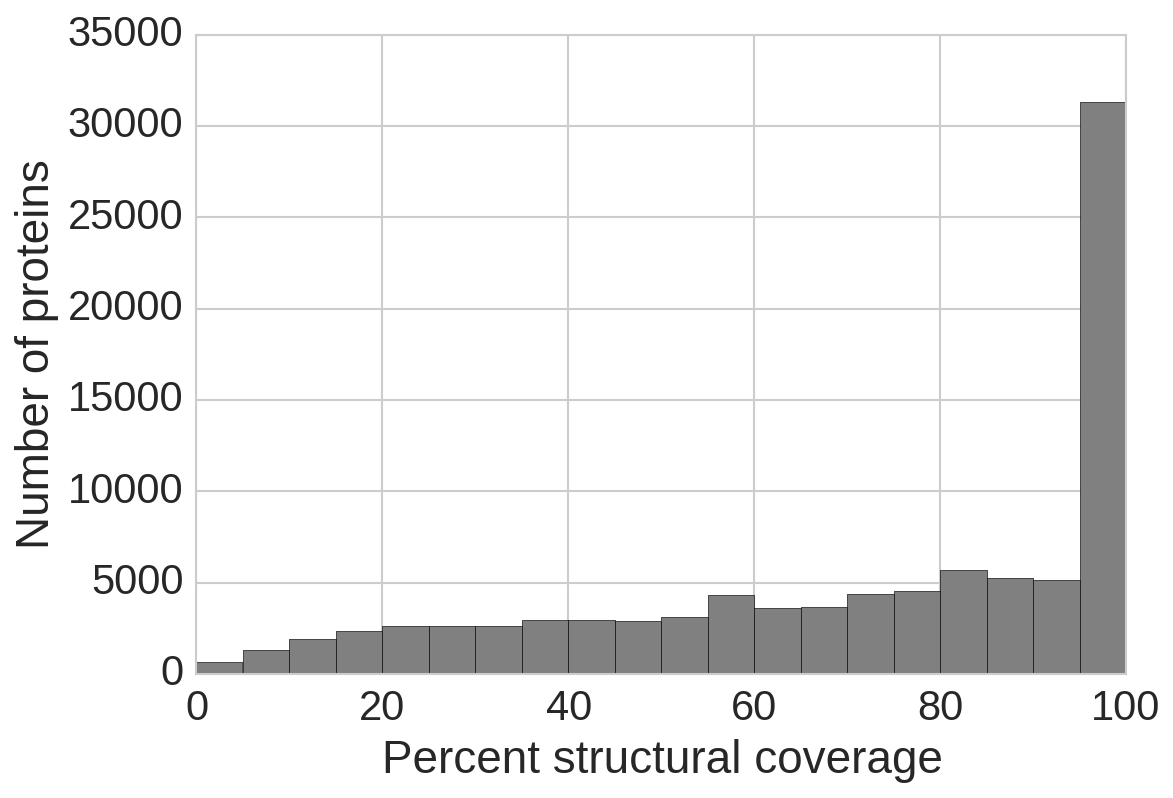
\includegraphics[scale=0.3]{elaspic_statistics/structural_coverage_hist}
	\caption{\textbf{Left}: statistics of how many homology models we were able to calculate. \textbf{Right}: structural coverage for proteins with at least one domain with a structural model.}
\end{figure}



\section{Comparing the energetic effect benign and deleterious mutations}



\section{Alanine scanning of protein-protein interfaces}




